\documentclass[oneside,final,a4 paper]{hcmut-report}
\usepackage{tabularx,microtype,xurl,needspace}
\usepackage[section]{placeins}
\usepackage{tikz}
\usetikzlibrary{arrows.meta,positioning}
\setlength{\parindent}{0 pt}
\setlength{\emergencystretch}{3 em}
\setlength{\headheight}{44.3 pt}
\setlength{\tabcolsep}{4 pt}
\captionsetup{font=small,labelfont=bf}
\newcommand{\cls}[1]{\texttt{\detokenize{#1}}}
\newcolumntype{Y}{>{\raggedright\arraybackslash}X}
\makeatletter
\renewcommand\small{\@setfontsize\small{11 pt}{13.2 pt}}
\renewcommand\footnotesize{\@setfontsize\footnotesize{10 pt}{12 pt}}
\makeatother
\deptname{Faculty of Computer Science and Engineering}
\coursename{Deep Learning and Its Applications (CO3133)}
\reporttype{ASSIGNMENT 2 -- M2 DRAFT}
\title{Video-Disjoint Semantic Segmentation of Marine Debris in TrashCan}
\advisor{Dr. Le Thanh Sach}
\groupname{Tiki-taka}
\reportplace{Ho Chi Minh City}
\reporttime{28 October 2026}
\logofile{hcmut.png}
\hypersetup{pdftitle={Tiki-taka A2 M2 Draft: Completed U-Net and Partial SegFormer Progress},pdfauthor={Nguyen Anh Khoa; Nguyen Hao Thien; Ta Tuan Khai}}

\begin{document}
\hypersetup{pageanchor=false}
\thispagestyle{empty}
\begin{center}
{\bfseries\fontsize{14}{17}\selectfont VIETNAM NATIONAL UNIVERSITY, HO CHI MINH CITY\par
HO CHI MINH CITY UNIVERSITY OF TECHNOLOGY\par
FACULTY OF COMPUTER SCIENCE AND ENGINEERING\par}
\vspace{0.8 cm}

\includegraphics[width=3cm]{hcmut.png}\par
\vspace{0.6 cm}
{\bfseries\fontsize{17}{21}\selectfont DEEP LEARNING AND ITS APPLICATIONS\par}
{\bfseries CO3133 -- SEMESTER-261\par}
\vspace{0.5 cm}
{\bfseries\fontsize{16}{20}\selectfont ASSIGNMENT 2 -- M2 DRAFT\par}
\vspace{0.5 cm}
{\bfseries\fontsize{20}{24}\selectfont Video-Disjoint Semantic Segmentation\par of Marine Debris in TrashCan\par}
\vspace{0.4 cm}
{\large Completed U-Net evaluation and partial SegFormer-B0 training\par}
\vspace{0.7 cm}
\begin{tabular}{rl}
\textbf{Class:} & CC01\\
\textbf{Instructor:} & Dr. Le Thanh Sach\\
\textbf{Group:} & Tiki-taka\\
\textbf{Milestone:} & M2 Draft\\
\textbf{Evidence cutoff:} & 28 October 2026
\end{tabular}\par
\vspace{0.5 cm}
\begin{tabular}{clc}\toprule
No. & Group member & Student ID\\\midrule
1 & Nguyen Anh Khoa & 2452539\\
2 & Nguyen Hao Thien & 2453194\\
3 & Ta Tuan Khai & 2452515\\\bottomrule
\end{tabular}
\vfill
{\bfseries Ho Chi Minh City, 28 October 2026}
\end{center}
\clearpage
\hypersetup{pageanchor=true}
\pagenumbering{roman}
\section*{Abstract}
\addcontentsline{toc}{section}{Abstract}
The project has completed a scratch U-Net experiment on a video-disjoint TrashCan-Material split and has progressed to pretrained SegFormer-B0: S0 has 15 completed main-training epochs, while S1 has completed its GPU pilot only.

The validation-selected U-Net checkpoint obtains test foreground mean intersection over union (mIoU) 0.035627 and foreground Dice 0.058519. The partial S0 run reaches best-so-far validation foreground mIoU 0.195336 at epoch 15; this is a validation progress result, not a SegFormer test result or a final model ranking.

The next stage is to complete S0, train the paired S1 configuration with color augmentation, and compare the two completed runs using the fixed validation rule before interpreting their test results. The current evidence does not establish the effect of augmentation or variability across seeds.

\vspace{0.4 cm}
\textbf{Keywords:} semantic segmentation; marine debris; TrashCan; U-Net; SegFormer; video-disjoint evaluation; progress report.
\clearpage
\tableofcontents
\clearpage
\pagenumbering{arabic}
\section{Problem and data description}
\subsection{Motivation and scope of this draft}
Underwater debris is difficult to distinguish from marine life and the seafloor because object appearance, scale, illumination and occlusion vary. TrashCan supplies underwater images with object-level annotations for marine debris research\cite{trashcan}. This project converts the polygons into a semantic segmentation task: each valid image pixel receives one class label, without distinguishing separate instances of the same class.

For an RGB image $x\in\mathbb{R}^{H\times W\times 3}$, the model predicts a map $\hat y\in\{0,\ldots,16\}^{H\times W}$. There are \textbf{17 output classes: background plus 16 foreground categories}. The foreground comprises ROV, plant, six animal categories and eight trash categories. Ignore label 255 is excluded from supervision and evaluation.

The research question is whether a pretrained modern segmentation model and modest photometric augmentation improve foreground overlap under a split that separates videos. This M2 draft reports the work completed through 28 October 2026: a completed U-Net experiment, an incomplete S0 SegFormer main run, and successful S0/S1 GPU pilots. It separates those observations from the remaining controlled comparison.

\subsection{Dataset source and provenance}
The working dataset is TrashCan 1.0 Material. The exploratory data analysis (EDA), measured on 5 October 2026, records 7,212 RGB images,12,336 polygon annotations and 312 filename-derived video groups. There are 3,245 images at $480\times 360$ and 3,967 at $480\times 270$. Source imagery is credited to JAMSTEC and the dataset to Hong, Fulton and Sattar\cite{trashcan}.

The source archive's license file and the annotation JSON license records are retained with the project evidence. The JSON records identify an Attribution-NonCommercial-ShareAlike entry; the archive also contains its own attribution and use statement. The report preserves both records rather than replacing them with an inferred license. Raw images, checkpoints and the large dataset archive are not redistributed in the report source package.

The instructor approved the proposal according to the project owner's confirmation on 26 October 2026. This statement records the confirmation used by the training setup; it is not an independently inspected learning-management-system submission record.

\subsection{Video-disjoint partition and class support}
The original source partitions contain 6,008 training images and 1,204 validation images. They share 127 filename-derived video IDs. Separating individual frames using those source labels would therefore allow frames from the same video into different evaluation partitions.

The project instead uses a fixed seed 36 manifest that assigns each video to exactly one partition. Metadata-based split construction uses deterministic greedy/local-search candidates, with at least three supporting training videos and two supporting videos in each held-out partition per foreground class. Table~\ref{tab:split} records the resulting image, video and annotation counts. Pairwise video-ID overlap is zero.
\begin{table}[H]
\centering\small
\caption{Fixed video-disjoint partition, split seed 36. Native mask percentages are retained from the 5 October 2026 EDA.}\label{tab:split}
\begin{tabular}{lrrrrr}\toprule
Partition & Images & Videos & Annotations & Background (\%) & Ignore (\%) \\ \midrule
Train & 5,057 & 207 & 8,563 & 89.13 & 0.0371 \\
Validation & 1,077 & 54 & 1,956 & 89.34 & 0.0754 \\
Test & 1,078 & 51 & 1,817 & 90.33 & 0.0238 \\
\bottomrule\end{tabular}
\end{table}

Video grouping addresses frame-level overlap under the chosen ID convention. It does not prove independence of dive locations or visually related scenes carrying different video IDs.

Class imbalance remains substantial after splitting. Table~\ref{tab:support} gives each foreground class's annotation count, video support and native supervised pixel totals. The small support for categories such as animal shells makes macro overlap and per-class results more informative than background-dominated accuracy.
\begin{table}[H]
\centering\small
\caption{Foreground class support in the fixed split. Pixel counts are native-resolution supervised pixels in millions, before letterboxing.}\label{tab:support}
\begin{tabular}{lrrrrrrr}\toprule
Class & Ann. & \multicolumn{3}{c}{Videos (train/val/test)} & \multicolumn{3}{c}{Pixels, M (train/val/test)} \\ \midrule
\cls{rov} & 3317 & 99 & 22 & 24 & 39.554 & 7.164 & 6.736 \\
\cls{plant} & 507 & 17 & 10 & 5 & 2.363 & 0.586 & 0.661 \\
\cls{animal_fish} & 764 & 33 & 7 & 5 & 4.421 & 1.444 & 1.577 \\
\cls{animal_starfish} & 398 & 9 & 3 & 3 & 0.123 & 0.037 & 0.022 \\
\cls{animal_shells} & 249 & 3 & 2 & 2 & 0.104 & 0.087 & 0.006 \\
\cls{animal_crab} & 309 & 9 & 3 & 3 & 0.789 & 0.199 & 0.196 \\
\cls{animal_eel} & 343 & 24 & 6 & 5 & 0.255 & 0.057 & 0.076 \\
\cls{animal_etc} & 235 & 12 & 6 & 7 & 0.805 & 0.079 & 0.177 \\
\cls{trash_etc} & 2039 & 107 & 23 & 23 & 9.145 & 1.921 & 1.601 \\
\cls{trash_fabric} & 314 & 14 & 4 & 3 & 2.285 & 0.422 & 0.352 \\
\cls{trash_fishing_gear} & 196 & 10 & 2 & 2 & 1.465 & 0.328 & 0.215 \\
\cls{trash_metal} & 1126 & 42 & 12 & 8 & 3.590 & 0.638 & 1.275 \\
\cls{trash_paper} & 193 & 6 & 2 & 2 & 0.947 & 0.257 & 0.056 \\
\cls{trash_plastic} & 1864 & 61 & 16 & 20 & 12.865 & 2.535 & 2.480 \\
\cls{trash_rubber} & 142 & 3 & 2 & 2 & 0.203 & 0.243 & 0.047 \\
\cls{trash_wood} & 340 & 14 & 3 & 3 & 2.900 & 0.467 & 0.332 \\
\bottomrule\end{tabular}
\end{table}

These counts describe dense native masks before resizing; they must not be mixed with the 512-canvas pixel totals reported by the evaluator.

The retained EDA figures provide a visual summary of the same imbalance and group coverage. Figure~\ref{fig:distribution} shows category frequencies, and Figure~\ref{fig:videos} shows support across video groups. Counts are from the 5 October audit rather than a new raw-data measurement in this report update.
\begin{figure}[H]\centering
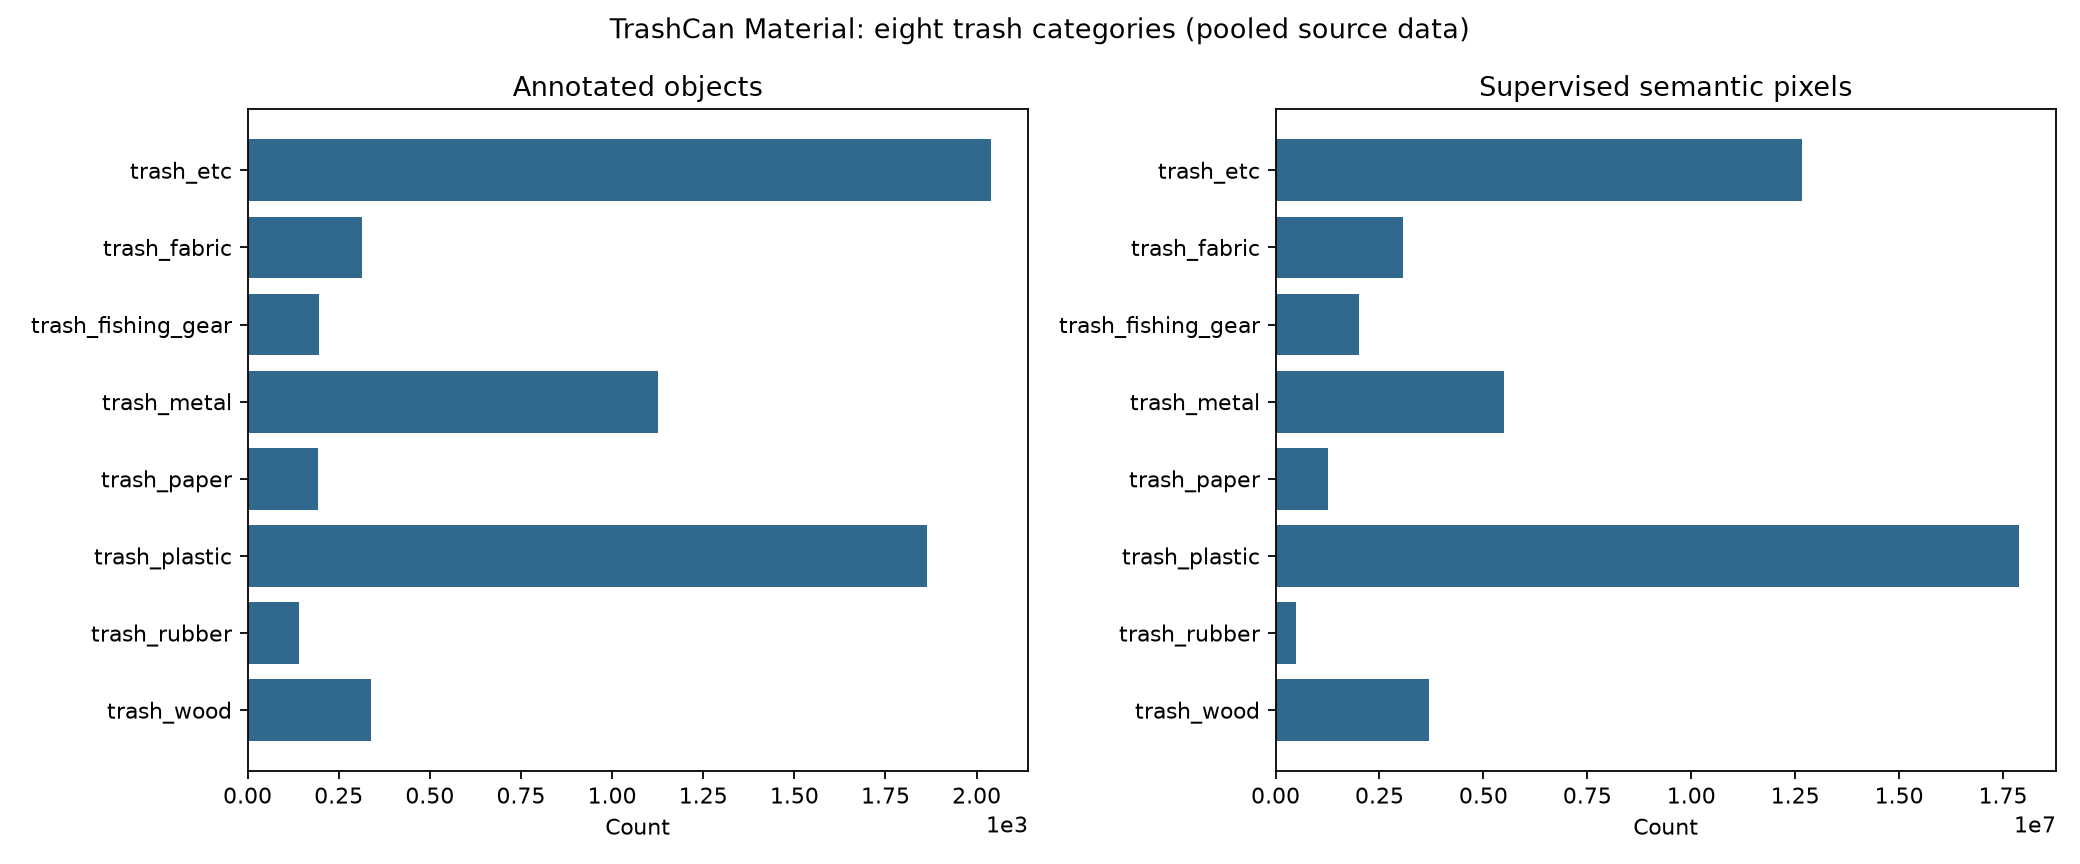
\includegraphics[width=.94\textwidth]{images/material_distribution.png}
\caption{Material-category distribution from the retained EDA.}\label{fig:distribution}
\end{figure}
\begin{figure}[H]\centering
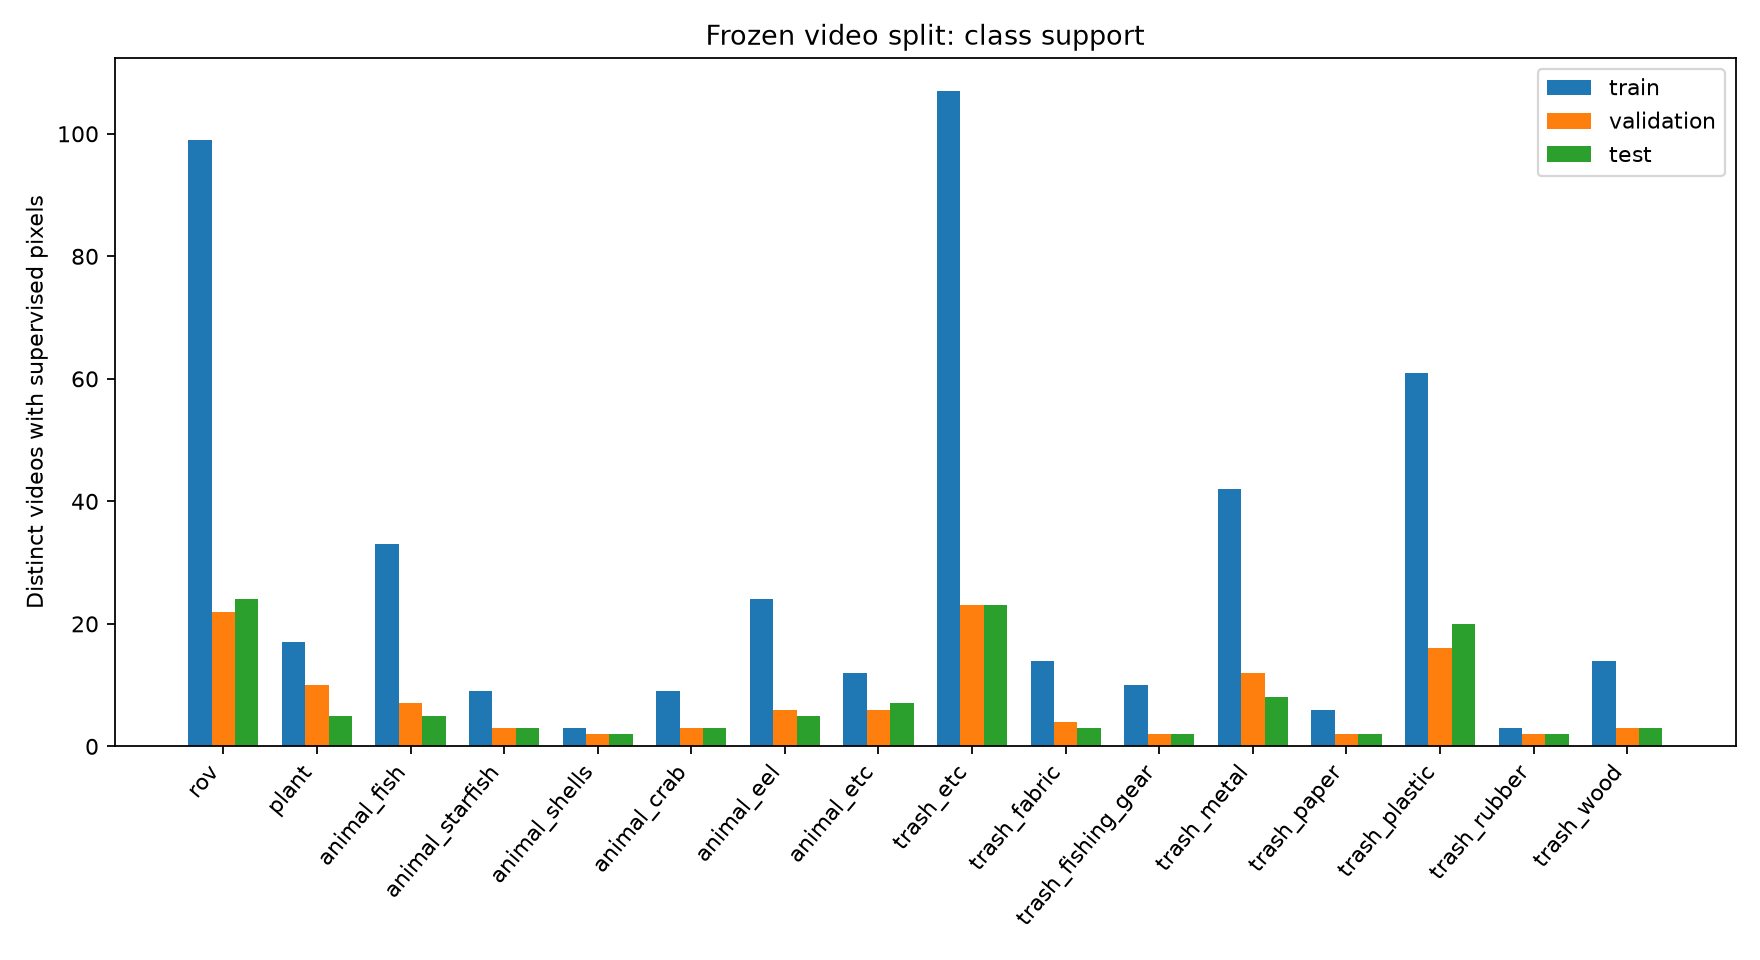
\includegraphics[width=.94\textwidth]{images/split_class_video_support.png}
\caption{Per-class video support under the fixed seed 36 split.}\label{fig:videos}
\end{figure}
The split provides class coverage in every partition while retaining rare classes; it does not remove their statistical uncertainty.

\subsection{Mask conversion, preprocessing and checks}
Polygons are rasterized on the native image canvas with Pillow 12.3.0. Same-class polygons are unioned; pixels where different foreground classes overlap receive ignore 255. Out-of-canvas regions are clipped. The EDA found no annotation that rasterized to an empty mask under this converter.

Each image is letterboxed to $512\times 512$ while preserving aspect ratio. RGB uses bilinear resizing, masks use nearest-neighbor resizing, RGB padding is black and target padding is ignore 255. The tensor is normalized with ImageNet channel means $(0.485,0.456,0.406)$ and standard deviations $(0.229,0.224,0.225)$. There is no label reduction or second image-processor resize.

The training adapter checks the published manifest digest, source annotation hashes, image dimensions, membership and native target hash. The supplied checks cover 5,057 training and 1,077 validation images. Figure~\ref{fig:qa} reproduces existing EDA annotation checks; it is not a gallery of model predictions.
At evaluation resolution, ignored pixels include the much larger letterbox padding region as well as native annotation conflicts. For example, U-Net test ignore fraction is 34.06\%; this does not mean that 34.06\% of the native annotations are conflicting.
\begin{figure}[H]\centering
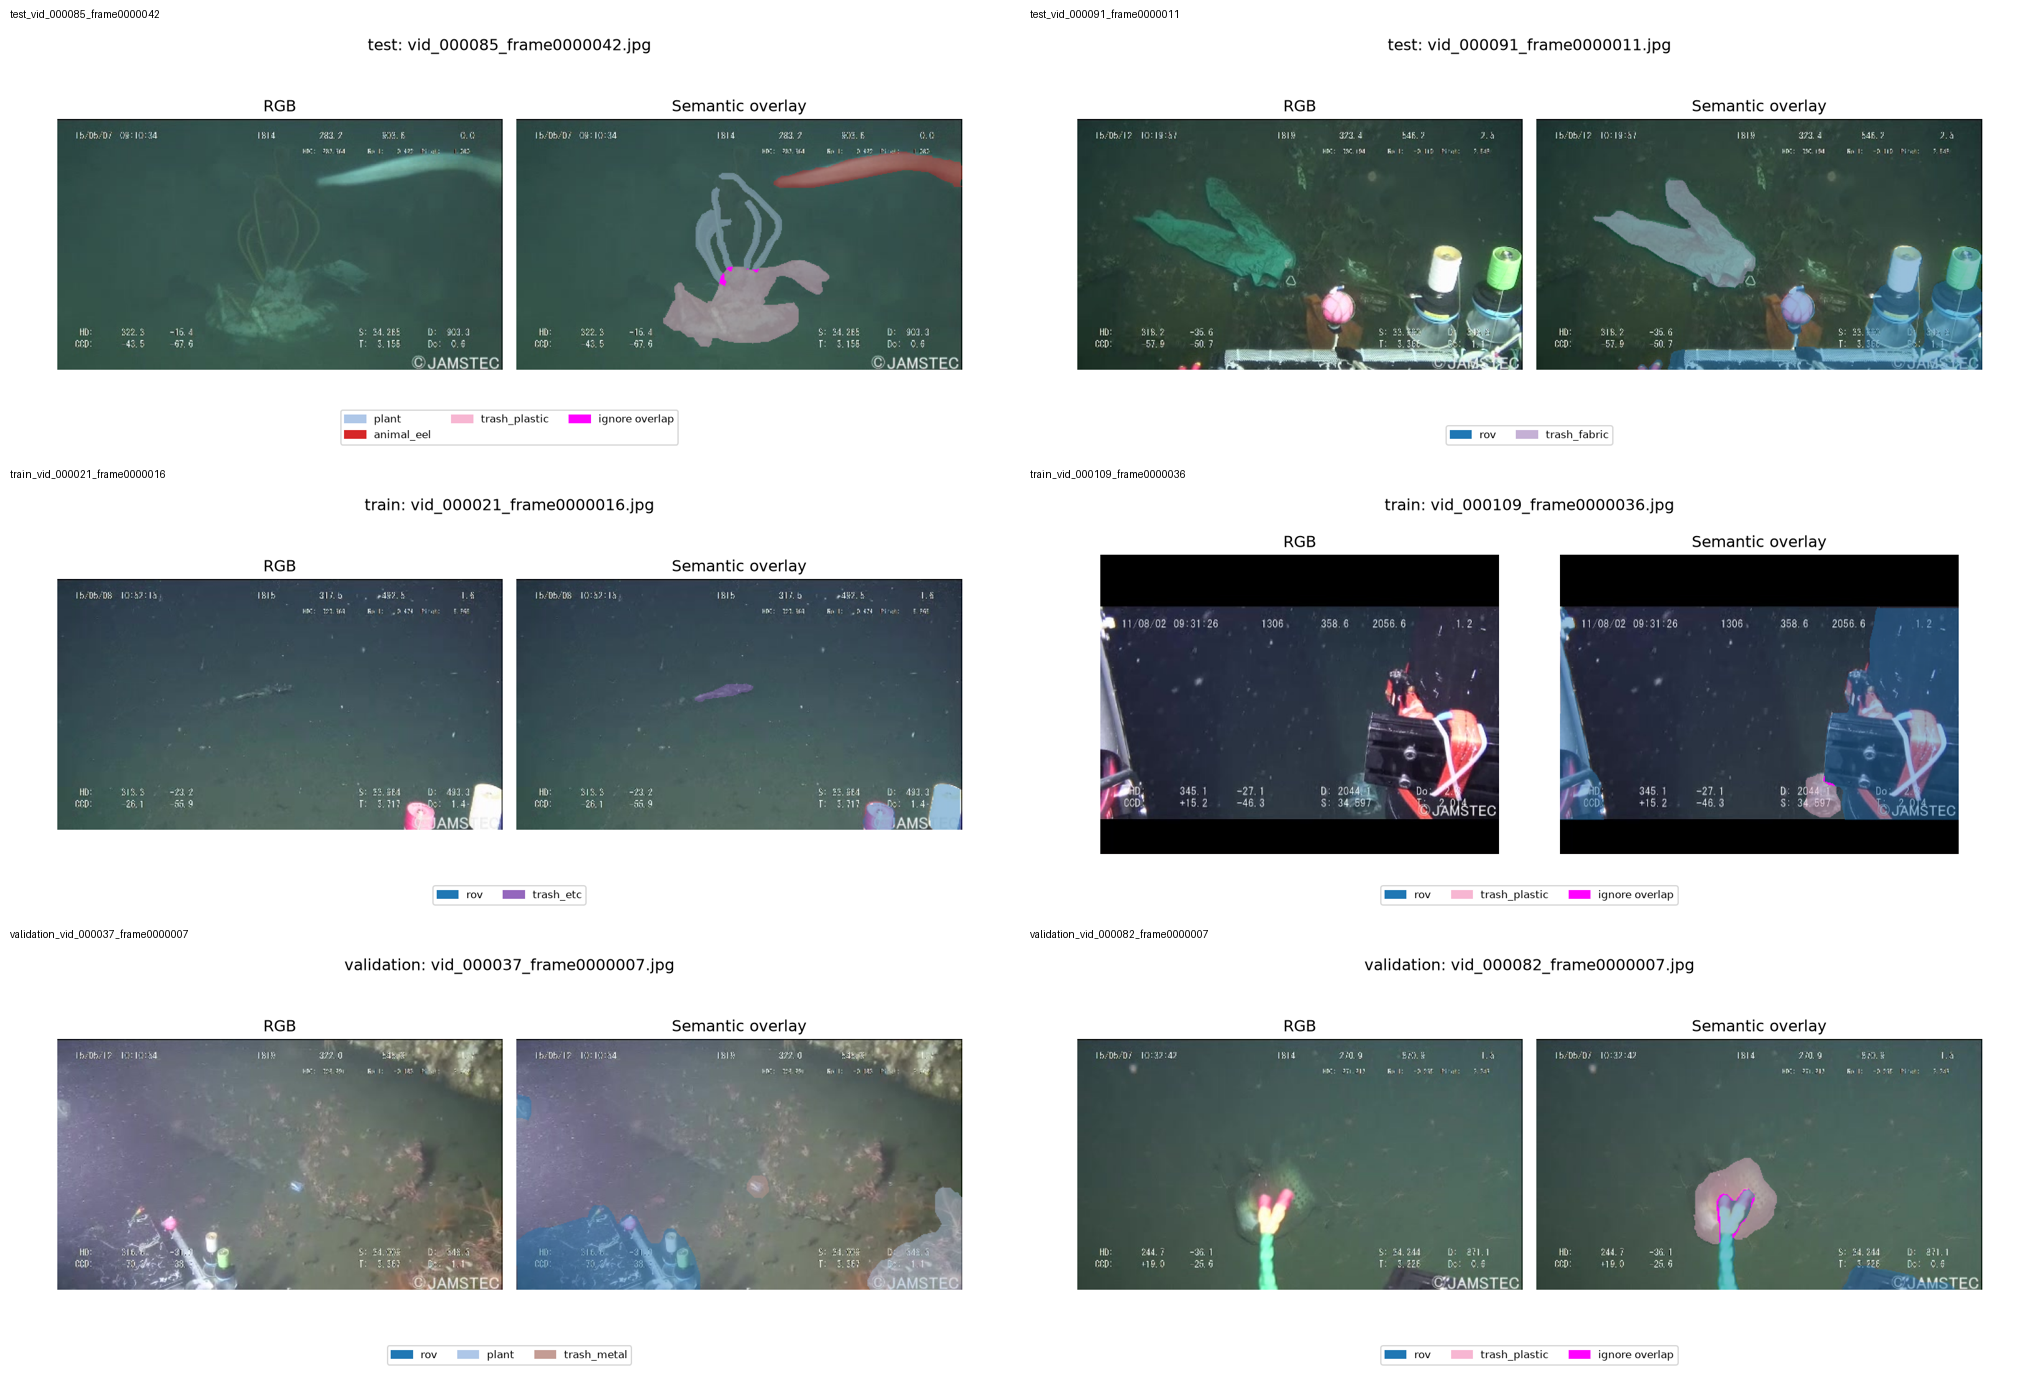
\includegraphics[width=.92\textwidth]{images/annotation_qa.png}
\caption{Six retained native annotation-QA examples, two per partition. RGB/mask overlays check conversion and alignment; they are ground truth, not inference outputs.}\label{fig:qa}
\end{figure}

\clearpage
\section{Methodology}
\subsection{Implemented pipeline}
The common pipeline keeps data conversion, objective and scoring consistent across models. Figure~\ref{fig:pipeline} shows the main flow; test data enters only the final evaluation stage of a completed run.
\begin{figure}[H]\centering
\begin{tikzpicture}[node distance=4 mm,box/.style={draw,rounded corners,align=center,text width=25 mm,minimum height=16 mm,font=\small},>=Latex]
\node[box](a){RGB and\linebreak polygons};
\node[box,right=of a](b){Rasterize;\linebreak video split};
\node[box,right=of b](c){Letterbox;\linebreak normalize};
\node[box,right=of c](d){U-Net or\linebreak SegFormer};
\node[box,right=of d](e){Train CE+Dice;\linebreak validate};
\node[box,below=7 mm of e](f){Select best;\linebreak evaluate test};
\draw[->](a)--(b);\draw[->](b)--(c);\draw[->](c)--(d);\draw[->](d)--(e);\draw[->](e)--(f);
\end{tikzpicture}
\caption{Shared segmentation workflow. Test scores do not select the training epoch.}\label{fig:pipeline}
\end{figure}
This separation makes the S0/S1 experiment a change to training RGB color augmentation while preserving the mask and evaluation conventions.

\subsection{Scratch U-Net baseline}
The compact U-Net follows an encoder--decoder design with skip connections\cite{unet}. The implemented version has four downsampling stages and channel widths 16,32,64,128,256. Each block contains two bias-free $3\times 3$ convolutions, eight-group Group Normalization and ReLU. Downsampling uses $2\times 2$ max pooling. The decoder upsamples bilinearly with \cls{align_corners=false}, concatenates encoder features, and applies another two-convolution block. A $1\times 1$ head produces 17 logits per pixel.

All 1,964,369 parameter elements are trainable, with zero frozen parameters. The model is initialized from scratch. Its completed run supplies the initial architecture baseline and the only model test result in the current snapshot.

\subsection{Pretrained SegFormer-B0 and full fine-tuning}
SegFormer combines a hierarchical Transformer encoder with a lightweight multilayer-perceptron decoder\cite{segformer}. The implementation loads \path{nvidia/segformer-b0-finetuned-ade-512-512}, pinned to revision \path{489d5cd81a0b59fab9b7ea758d3548ebe99677da}. The pretrained encoder and compatible decoder weights are retained, while the 150-class ADE20K classifier is replaced by a newly initialized 17-class classifier.

The complete model is fine-tuned end to end: encoder, decoder and classifier parameters all receive updates. Total and trainable counts are both 3,718,513; frozen count is zero. Pretrained initialization therefore does not imply a frozen backbone. Lower-resolution raw logits are bilinearly interpolated to the 512-canvas target before computing loss and argmax predictions.

S0 and S1 are initialized independently from the same checkpoint and seed 69420. Only S0 currently has main-run metadata, so equality of the two actual main initial-state hashes cannot yet be established from this snapshot. The setup checks this equality once both main-run records exist; the earlier synthetic authoring check is separate from that future run-level check.

\subsection{Objective and evaluation metrics}
Training minimizes the sum of multiclass cross-entropy and foreground soft Dice loss, each with coefficient 1:
\begin{equation}
\mathcal L=\mathcal L_{\mathrm{CE}}+\frac{1}{|C_B|}\sum_{c\in C_B}\left(1-\frac{2\sum_{i\in V_B}p_{ic}y_{ic}+\epsilon}{\sum_{i\in V_B}(p_{ic}+y_{ic})+\epsilon}\right).
\end{equation}
Here $V_B$ is the set of valid pixels in a batch, $C_B$ contains foreground classes with target support in that batch, $p_{ic}$ is the softmax probability, $y_{ic}$ is the one-hot target and $\epsilon=10^{-6}$. Cross-entropy ignores 255. A batch with no foreground contributes zero Dice loss; an all-ignore batch is skipped for optimization. Logged epoch loss is a valid-pixel-weighted average of batch objectives, not a Dice score calculated from the epoch confusion matrix.

For hard predictions, the evaluator accumulates one 17-by 17 confusion matrix across the whole partition. For class $c$,
\begin{equation}
\operatorname{IoU}_c=\frac{TP_c}{TP_c+FP_c+FN_c},\qquad
\operatorname{Dice}_c=\frac{2TP_c}{2TP_c+FP_c+FN_c}.
\end{equation}
Rows are ground truth and columns are predictions. Foreground mIoU/Dice average IDs 1--16; trash mIoU averages IDs 9--16. All-class metrics include background. Undefined denominators are omitted and the number of defined classes is recorded. All 16 foreground classes have defined IoU in the reported held-out scores, including classes with zero intersection. Pixel accuracy divides the confusion diagonal by all valid pixels.

\subsection{Training budget, checkpointing and environment}
Both model families use AdamW, weight decay 0.01, batch 4, up to 40 epochs, patience 8, FP 32, no learning-rate scheduler and no mixed precision. U-Net learning rate is $10^{-3}$; SegFormer uses $6\times 10^{-5}$. Training seed 69420 is distinct from split seed 36. The training loader shuffles with a separate generator seeded by run seed plus epoch; validation/test are unshuffled.

The best checkpoint maximizes validation foreground mIoU; a tie uses lower validation loss, then the earlier epoch. Each completed epoch saves model, AdamW state, random-number states, history, best selection and early-stopping counter. Resume restores this state; an incomplete epoch is repeated. The U-Net continuation belongs to the same experiment and is not an independent seed.

The supplied runs/pilots record a Tesla T4 with 14.56 GiB memory, Python 3.13.16, PyTorch 2.11.0+cu 130, torchvision 0.26.0+cu 130 and NumPy 2.1.3. Pillow 12.3.0 and Transformers 4.57.6 are pinned. TF 32 is disabled and CUDA deterministic algorithms use warning-only mode for the bilinear-backward limitation. These settings and saved RNG state do not promise cross-runtime GPU bitwise identity.

\subsection{Controlled factor and current execution status}
S0 disables color jitter. S1 applies it to training RGB with probability 0.5: brightness, contrast and saturation factors are sampled in $[0.9,1.1]$, hue shift in $[-0.01,0.01]$, with shuffled operation order. Masks are unchanged. A seed/epoch/image-specific random stream keeps augmentation separate from model and sampling randomness. There is no geometric augmentation; held-out images are unaugmented.

The paired setup locks both configurations and their numerical environment before main training or test evaluation. S0/S1 share architecture, pretrained revision, seed, split, normalization, optimizer, learning rate, loss and budget. Run name and train color switch are their only treatment differences. Table~\ref{tab:status} distinguishes planned settings from completed execution.
\begin{table}[H]\centering\small
\caption{Experiment status at the supplied 28 October snapshot.}\label{tab:status}
\begin{tabularx}{\textwidth}{lYY}\toprule
Configuration & Completed evidence & Status of remaining work\\\midrule
U: scratch U-Net &23 epochs, early stopping; best 15; validation and test scored & Main/test complete for seed 69420\\
S0: pretrained B0, color off &20-step pilot;15 main epochs; best-so-far 15 & Main incomplete; no test result\\
S1: pretrained B0, color on &20-step pilot; frozen configuration & Main not started in supplied snapshot\\
Constant background & Metrics derived analytically from held-out supports & No trainable model or inference run\\\bottomrule
\end{tabularx}
\end{table}
The S0/S1 hypothesis is that mild color changes improve held-out foreground overlap. It cannot yet be tested because S1 has no main-training result. U versus S0 is a descriptive comparison of model configurations: architecture, initialization and learning rate change together, and the current training completion states differ. It does not isolate the causal effect of pretraining.

\clearpage
\section{Implementation results at the current snapshot}
\subsection{Completed U-Net training and evaluation}
The U-Net experiment completed 23 epochs and stopped after eight consecutive epochs without an improved validation foreground mIoU. Its selected checkpoint is epoch 15. This includes an epoch-boundary continuation from epoch 7 after host kernel/RAM descriptors changed; the continuation retains the same experiment, seed and budget.

Figure~\ref{fig:unetcurves} shows training loss decreasing from 1.5083 at epoch 1 to 0.6102 at epoch 23 while training foreground mIoU rises from 0.0132 to 0.4072. Validation foreground mIoU peaks at 0.053085 at epoch 15; its final value is 0.047450. Validation loss is lowest at epoch 5 (1.271954) and ends at 1.516843. The growing train--validation gap is consistent with overfitting in this run, without establishing a single cause.
\begin{figure}[H]\centering
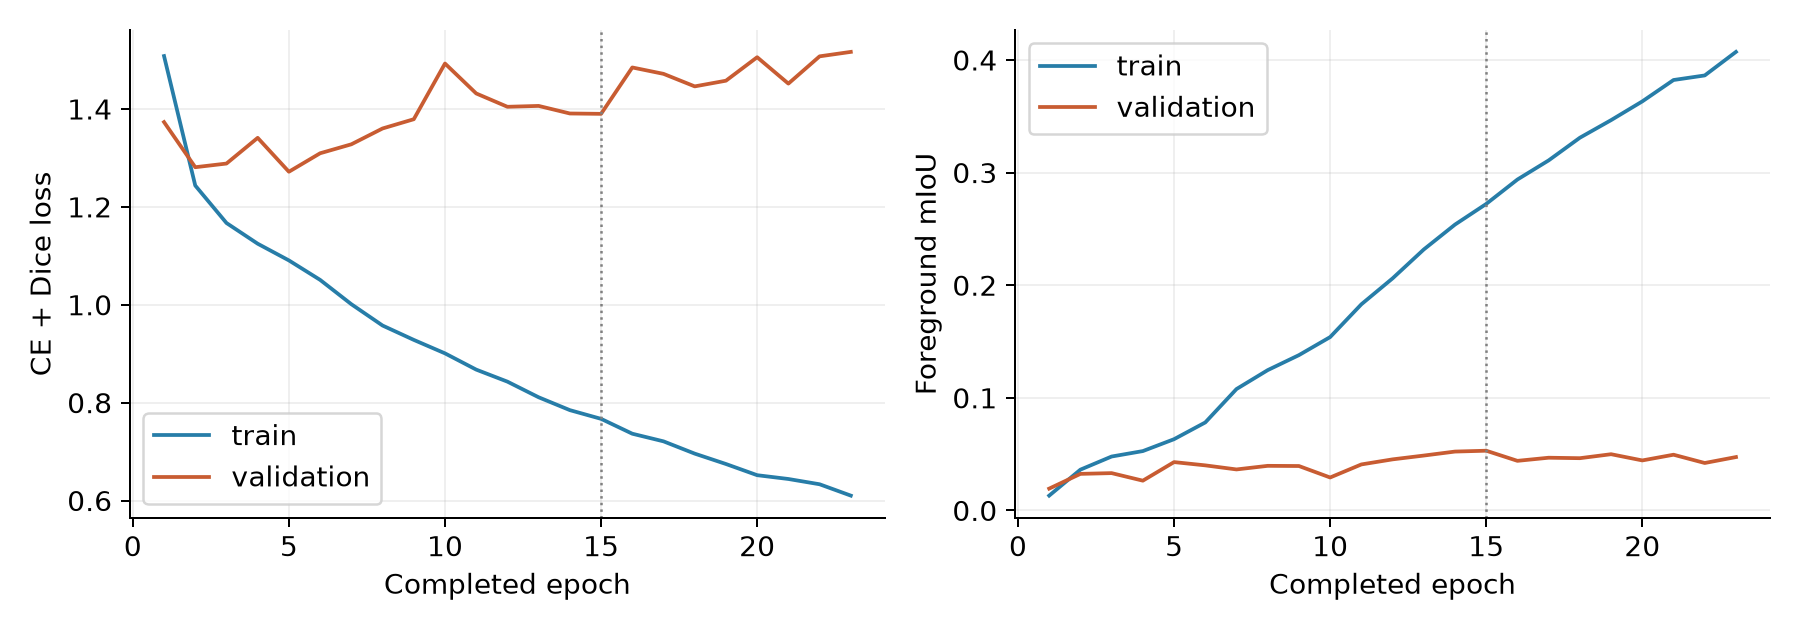
\includegraphics[width=\textwidth]{images/unet_curves.png}
\caption{Completed U-Net history. The dotted line marks the validation-selected epoch 15; the run ends at epoch 23.}\label{fig:unetcurves}
\end{figure}
The metric used to choose the checkpoint is foreground mIoU, so minimum validation loss and selected epoch need not coincide.

The selected checkpoint was replayed on validation and evaluated on all 1,078 test images. Table~\ref{tab:metrics} places these completed U-Net scores next to S0's best-so-far validation score, while retaining the different execution states.
\begin{table}[H]
\centering\small
\caption{Measured metrics at epoch 15. U-Net is a completed run; S0 is a15-epoch partial snapshot. All scores are on a0--1 scale.}\label{tab:metrics}
\begin{tabular}{lrrr}\toprule
Metric & U validation & U test & S0 validation \\ \midrule
Foreground mIoU & 0.053085 & 0.035627 & 0.195336 \\
Foreground Dice & 0.084369 & 0.058519 & 0.280506 \\
Trash mIoU & 0.032704 & 0.014652 & 0.137865 \\
All-class mIoU & 0.103646 & 0.087050 & 0.239732 \\
All-class Dice & 0.135542 & 0.111123 & 0.321323 \\
CE + Dice loss & 1.390246 & 1.407840 & 1.134105 \\
Valid pixels (M) & 176.765 & 186.340 & 176.765 \\
Ignored pixels (\%) & 37.39 & 34.06 & 37.39 \\
\bottomrule\end{tabular}
\end{table}

U-Net test foreground mIoU is 0.035627, foreground Dice 0.058519 and trash mIoU 0.014652. Its validation-to-test foreground mIoU difference is 0.017458. These are observations for a single seed and fixed split, rather than estimates of variability across repeated runs.

\subsection{Measured SegFormer pilots}
Both SegFormer arms completed 20 optimization steps on a fixed real training batch before their main configurations were frozen. Table~\ref{tab:pilots} records finite-loss, gradient and capacity diagnostics. Each pilot's final loss is lower than its initial loss, and peak reserved CUDA memory remains below 90\% of GPU memory.
\begin{table}[H]
\centering\small
\caption{Measured 20-step, fixed-train-batch diagnostics on the T4. These are capacity/gradient checks, not held-out segmentation results.}\label{tab:pilots}
\begin{tabular}{lrrrr}\toprule
Arm & First loss & Last loss & Peak reserved (GiB) & GPU memory (GiB) \\ \midrule
S0 & 3.8140 & 3.0349 & 2.70 & 14.56 \\
S1 & 3.8145 & 3.0304 & 2.73 & 14.56 \\
\bottomrule\end{tabular}
\end{table}

Pilot models are discarded; main training starts again from the prescribed pretrained checkpoint and seed. The similar pilot losses do not measure the effect of augmentation on held-out segmentation. Pilot memory is also not a measurement of peak memory across the complete main-training workload.

\subsection{S0 main-training progress: 15 completed epochs}
The supplied S0 checkpoint/history contains 15 completed epochs, below the configured 40-epoch limit. Epoch 15 is currently best, and the early-stopping counter is zero. Therefore the snapshot is \textbf{an incomplete main run}, not a completed 40-epoch or early-stopped SegFormer experiment.

Figure~\ref{fig:s0 curves} shows the available S0 history. Training loss falls from 1.250555 at epoch 1 to 0.247658 at epoch 15, and training foreground mIoU rises from 0.084281 to 0.744726. Validation foreground mIoU rises from 0.100556 to its current maximum 0.195336. At epoch 15, validation Dice is 0.280506, trash mIoU 0.137865 and loss 1.134105.
\begin{figure}[H]\centering
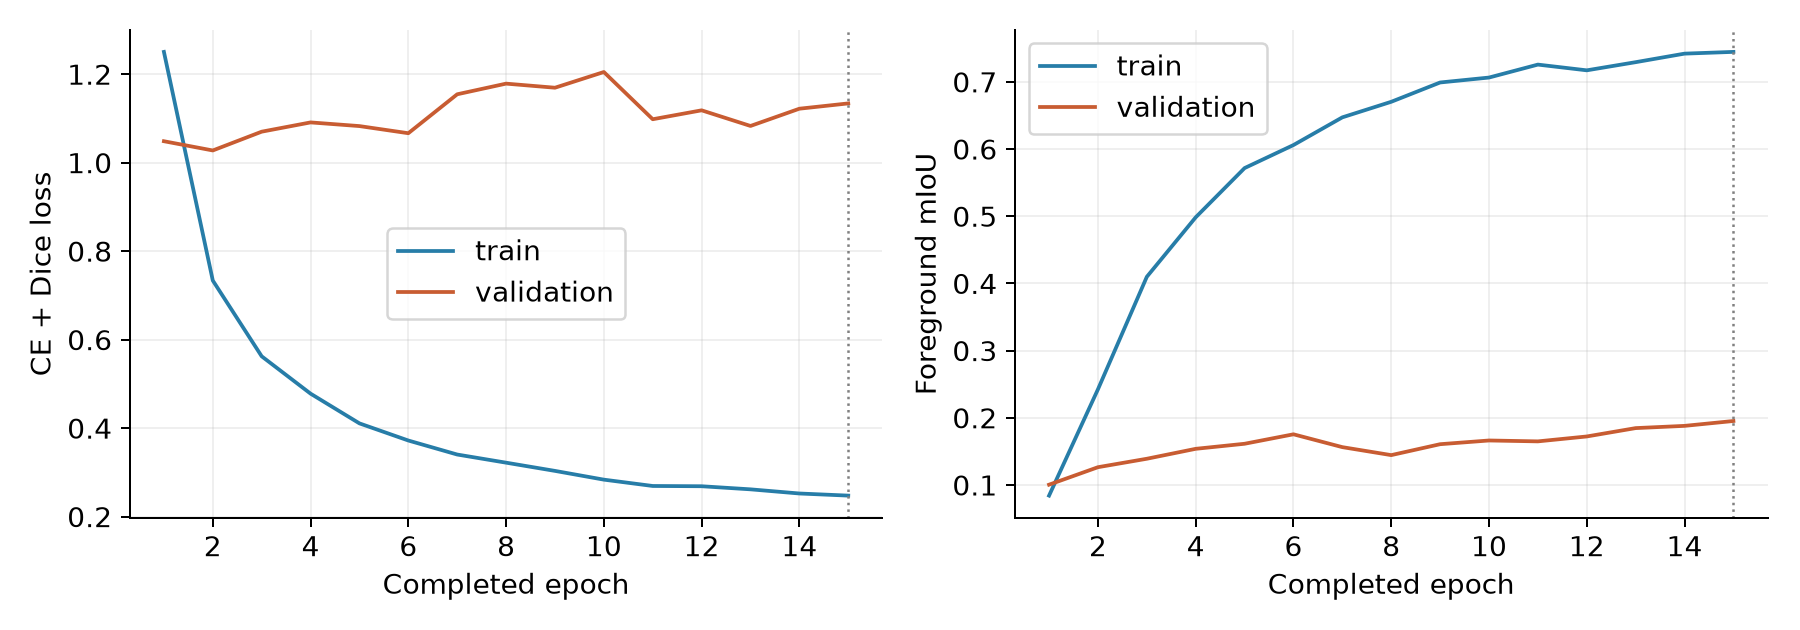
\includegraphics[width=\textwidth]{images/segformer_s0_curves.png}
\caption{Partial SegFormer S0 history through epoch 15. The selected epoch is best-so-far; training has not reached its completion criterion.}\label{fig:s0 curves}
\end{figure}
The latest train--validation foreground mIoU gap is 0.549390. Validation loss reached its lowest observed value at epoch 2 (1.027752), whereas foreground mIoU is highest at epoch 15. Better hard-mask overlap and lower probabilistic loss need not occur together; the saved foreground-mIoU selection rule remains unchanged. The large training/validation gap motivates continued scrutiny of class generalization, rather than treating the training score as held-out quality.

The partial S0 validation mIoU exceeds the completed U-Net validation mIoU by 0.142251 (14.2251 percentage points). This comparison uses the same validation membership and scoring convention. It is evidence that the current S0 configuration learns useful foreground structure; architecture, initialization, learning rate and execution progress differ, so it is neither a final ranking nor a controlled estimate of pretraining's contribution. No S0 test score or independent best-checkpoint validation replay is included in the supplied snapshot; the S0 values come from completed epoch validation in the training history.

\subsection{Per-class overlap and error patterns}
Table~\ref{tab:perclass} preserves each class's measured overlap, and Figure~\ref{fig:classcompare} compares only the two validation columns. The U test column remains a separate completed held-out evaluation.
\begin{table}[H]
\centering\small
\caption{Class-wise overlap. S0 columns use its best-so-far validation checkpoint; no S0 test result is claimed.}\label{tab:perclass}
\begin{tabular}{rlrrrr}\toprule
ID & Class & U val IoU & U test IoU & S0 val IoU & S0 val Dice \\ \midrule
0 & \cls{background} & 0.9126 & 0.9098 & 0.9501 & 0.9744 \\
1 & \cls{rov} & 0.4722 & 0.3564 & 0.6907 & 0.8171 \\
2 & \cls{plant} & 0.0190 & 0.0038 & 0.1074 & 0.1940 \\
3 & \cls{animal_fish} & 0.0162 & 0.0367 & 0.5031 & 0.6694 \\
4 & \cls{animal_starfish} & 0.0000 & 0.0000 & 0.0323 & 0.0627 \\
5 & \cls{animal_shells} & 0.0000 & 0.0000 & 0.0000 & 0.0000 \\
6 & \cls{animal_crab} & 0.0804 & 0.0292 & 0.2820 & 0.4399 \\
7 & \cls{animal_eel} & 0.0000 & 0.0268 & 0.4068 & 0.5784 \\
8 & \cls{animal_etc} & 0.0000 & 0.0000 & 0.0000 & 0.0000 \\
9 & \cls{trash_etc} & 0.0802 & 0.0325 & 0.0575 & 0.1088 \\
10 & \cls{trash_fabric} & 0.0358 & 0.0145 & 0.0729 & 0.1359 \\
11 & \cls{trash_fishing_gear} & 0.0000 & 0.0000 & 0.0078 & 0.0155 \\
12 & \cls{trash_metal} & 0.0390 & 0.0036 & 0.0618 & 0.1163 \\
13 & \cls{trash_paper} & 0.0000 & 0.0000 & 0.1849 & 0.3121 \\
14 & \cls{trash_plastic} & 0.0901 & 0.0666 & 0.2474 & 0.3966 \\
15 & \cls{trash_rubber} & 0.0000 & 0.0000 & 0.0012 & 0.0024 \\
16 & \cls{trash_wood} & 0.0166 & 0.0000 & 0.4694 & 0.6389 \\
\bottomrule\end{tabular}
\end{table}

S0's strongest foreground validation IoUs at epoch 15 are ROV 0.6907, animal fish 0.5031, trash wood 0.4694 and animal eel 0.4068. Animal shells and animal other still have zero validation IoU. Improvement is not uniform: trash other has S0 validation IoU 0.0575 compared with U-Net 0.0802. A higher macro score therefore does not imply every debris category has improved.
\begin{figure}[H]\centering
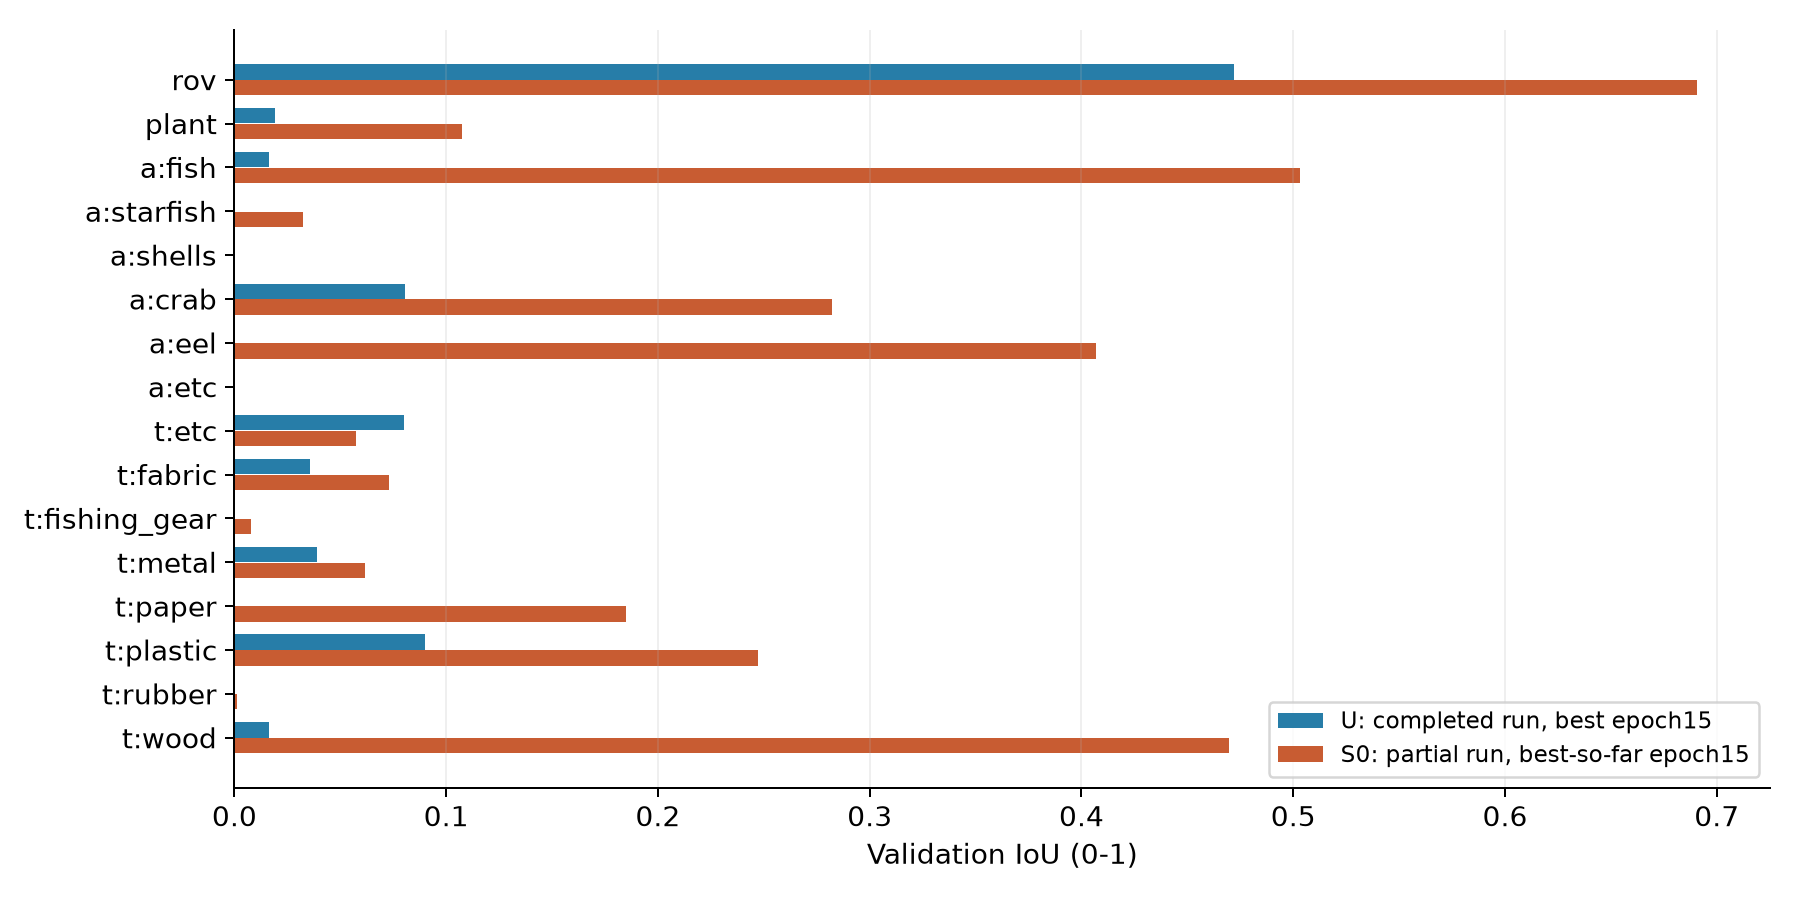
\includegraphics[width=\textwidth]{images/validation_per_class.png}
\caption{Validation IoU by foreground class. U is a completed run and S0 is partial; both columns refer to epoch 15. Prefixes a:/t: denote animal/trash.}\label{fig:classcompare}
\end{figure}
The U-Net test result remains weak across many categories: six foreground classes have zero IoU, and its strongest foreground class is ROV (0.3564). Sparse support is a plausible contributor, but aggregate counts do not distinguish class imbalance, appearance shift, boundary errors and optimization effects as causes.

To show how these errors are distributed, Figure~\ref{fig:confusion} normalizes each confusion row by its true-class support. This puts frequent and rare categories on a common within-class scale. The left panel is U test; the right is S0 validation, so the panels are not a same-partition model comparison.
\begin{figure}[H]\centering
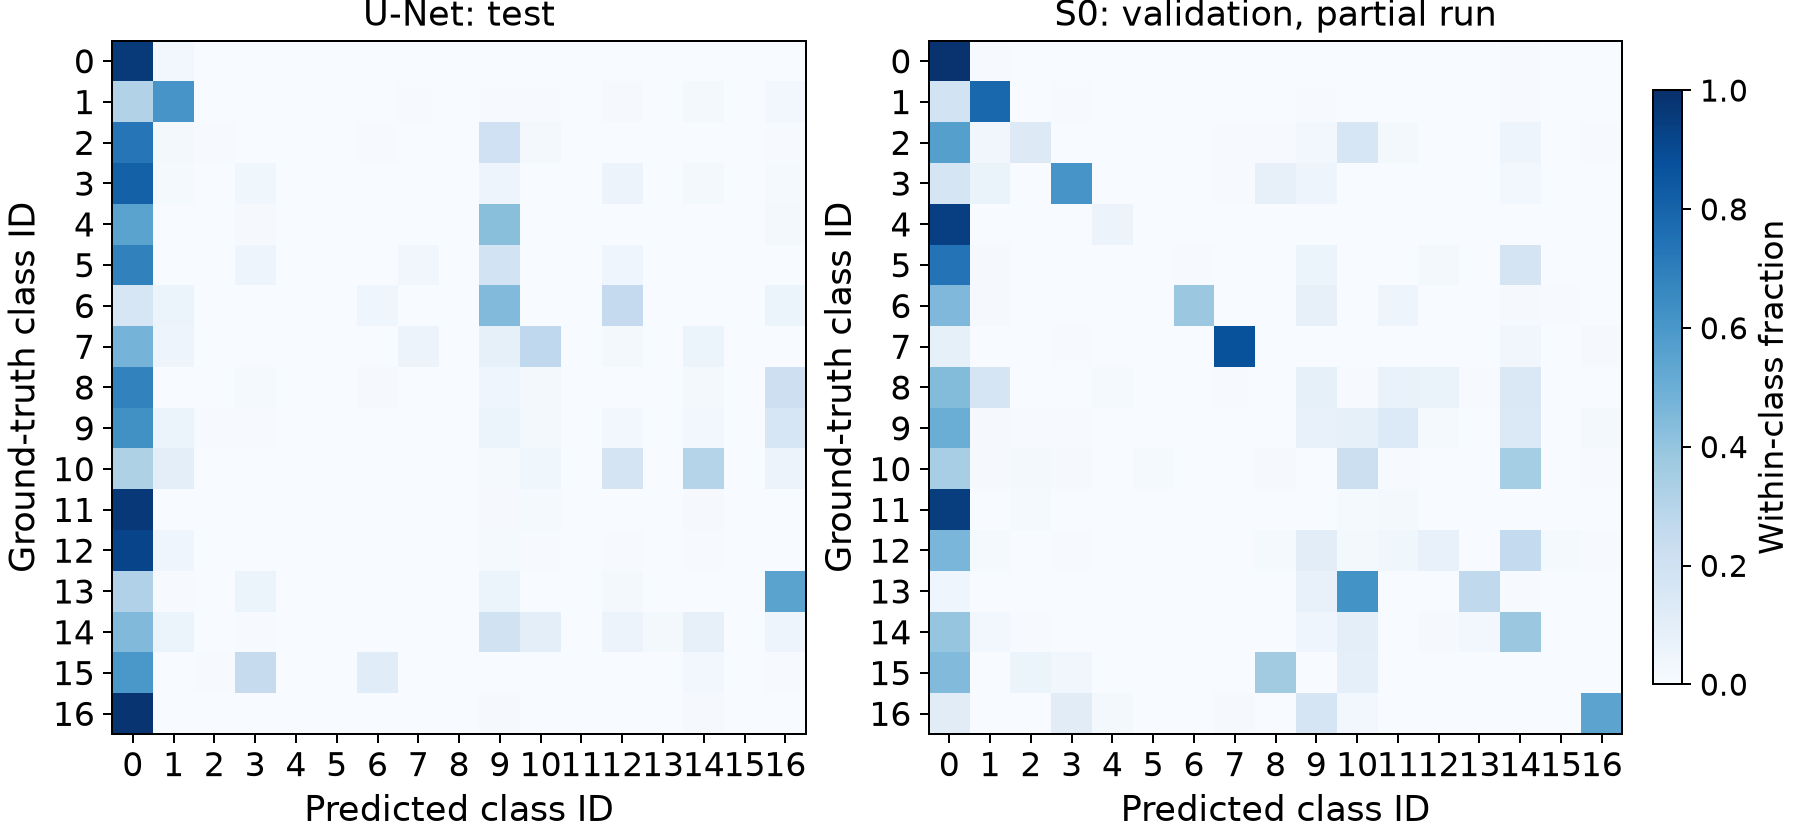
\includegraphics[width=\textwidth]{images/confusion_panels.png}
\caption{Row-normalized confusion: U-Net test (left) and partial S0 validation (right). Both color scales run 0--1; class IDs are defined in Table~\ref{tab:perclass}.}\label{fig:confusion}
\end{figure}
In the U test matrix,9,174,492 of 17,988,134 foreground pixels (51.00\%) are assigned to background. This directly measures foreground omission. It does not identify whether the missed pixels correspond to small objects, occlusion or particular visual conditions; that requires prediction-level image inspection.

\subsection{Analytical background-only reference}
A predictor that assigns every valid pixel to background provides a useful check on the interpretation of accuracy. Its confusion matrix can be constructed without inference: place each true-class support in column 0. Table~\ref{tab:background} derives this reference from the already saved held-out confusion-row totals; it is an analytical calculation on existing labels, not a newly trained model or an additional checkpoint evaluation.
\begin{table}[H]
\centering\small
\caption{Analytical constant-background reference derived from existing confusion-row supports; no model inference is required.}\label{tab:background}
\begin{tabular}{lrrrr}\toprule
Partition / predictor & Pixel acc. & FG mIoU & FG Dice & All mIoU \\ \midrule
Validation / background & 0.894015 & 0.000000 & 0.000000 & 0.052589 \\
Test / background & 0.903466 & 0.000000 & 0.000000 & 0.053145 \\
Test / U-Net & 0.894205 & 0.035627 & 0.058519 & 0.087050 \\
\bottomrule\end{tabular}
\end{table}

On test, constant background obtains pixel accuracy 0.903466, above U-Net's 0.894205, yet has foreground mIoU and Dice exactly zero. U-Net's nonzero foreground overlap and higher all-class mIoU show a different trade-off. This establishes why the study uses foreground macro metrics as primary outcomes: pixel accuracy alone can favor a predictor that never finds debris or marine-life classes.

\subsection{Compute records and qualitative evidence boundary}
S0's supplied progress log contains 15 training-phase records totaling 14,243.52 seconds (3.9565 hours) and 15 validation records totaling 838.61 seconds (13.98 minutes). These are phase durations for the 15 completed epochs, excluding setup, pilots, checkpoint writes, idle/disconnected time and final test processing. They are not complete-experiment wall time or inference latency. No inference benchmark is reported, and a completed U/S0 cost comparison is deferred until both scopes can be reconciled.

The current report includes annotation-QA overlays and aggregate confusion evidence. It does not present ground-truth overlays as model predictions. Prediction galleries, including foreground misses and inter-class confusions, will be exported from selected checkpoints after the respective run completes; no new checkpoint inference was performed during this report update.

\subsection{S1 status and the pending augmentation comparison}
S1 has a successful GPU pilot and a frozen color-on configuration, but the supplied S1 folder contains no main-run directory, epoch history or main checkpoint. Consequently there is no S1 validation/test score to compare with S0, no main-run initial-state hash pair to verify yet, and no observed augmentation effect.

The experiment remains defined as S0 versus S1 with the same architecture, initialization scheme, seed, split, optimizer, learning rate and budget. Completing this pair is the next experiment milestone; the 20-step pilot is not substituted for that comparison.

\clearpage
\section{Limitations and next experiments}
The evidence covers one completed U-Net run and one partial SegFormer S0 run, each at seed 69420. SegFormer test performance, the S0/S1 augmentation effect and multi-seed variability remain outside the measured results. The current S0 validation lead must not be interpreted as a generalization guarantee or a causal estimate of pretraining.

Video-disjoint membership prevents the measured 127 source video-ID overlaps, but filename-derived IDs do not establish independence of dives, locations or scenes. The semantic conversion ignores cross-class conflicts and discards instance identities. Letterboxing and class imbalance also affect what the reported pixel counts and overlap scores represent. The two zero-IoU S0 validation classes and the U-Net foreground misses remain substantive limitations despite improvements in other classes.

The next steps are sequenced to preserve the comparison:
\begin{enumerate}
\item Resume S0 from the saved epoch 15 state until the existing budget or early-stopping condition is reached. Retain the original settings and select best using validation foreground mIoU.
\item Train S1 from its prescribed pretrained initialization with only train color augmentation changed. Verify equality of the actual main initial-state hashes and compatibility of the numerical environments before interpreting the paired contrast.
\item Evaluate completed selected checkpoints with the existing fixed test stage, then report the two arms separately. Test results describe the completed configurations and must not guide changes to this pair.
\item Compare foreground mIoU/Dice and class-level changes; export prediction galleries to inspect foreground omission and rare-category failures. If compute permits, repeat the paired comparison with the prespecified additional seeds 67 and 69 to quantify seed variation.
\item Measure inference cost using the same device, input shape, precision, batch size and timing definition. Keep those measurements separate from epoch-phase and pilot timings.
\end{enumerate}
If runtime resources are limited, executing S0 and S1 in separate sessions with the same pair tag and locked environment preserves the intended factor better than silently changing batch size or resolution in one arm. A deliberate protocol change requires a new pair and separately reported settings.

\section{Conclusion}
The project has moved beyond implementation setup. It has a verified video-disjoint data pipeline, a completed scratch U-Net training/test experiment, two successful SegFormer GPU pilots, and 15 completed epochs of pretrained SegFormer S0 main training.

U-Net selects epoch 15 after 23 completed epochs and reaches test foreground mIoU 0.035627 and Dice 0.058519. The incomplete S0 run reaches best-so-far validation mIoU 0.195336 at epoch 15, compared with U-Net validation 0.053085. The current S0 result is promising at the configuration level, while large train--validation gaps and persistent rare-class failures show that segmentation quality remains uneven.

This M2 draft establishes current progress, not a completed architecture or augmentation study. Completing S0 and S1, preserving validation-based selection, and then evaluating the selected checkpoints are required before answering whether the planned color augmentation helps. Robustness across seeds and inference-cost trade-offs remain subsequent measurements.

\section{Reproducibility and evidence record}
\subsection{Source, effective configuration and provenance}
The supplied U and S0 run records use source revision
\begin{quote}\small\path{7df323698d1ae4d5122850a54eb38b01609d80f1}\end{quote}
and source digest
\begin{quote}\small\path{13ea100cefed8e7bd13c38153ebd3321760804366e2b5a66b47d2076d7e0c503}.\end{quote}
The manifest canonical digest is
\begin{quote}\small\path{87905f1a97dd2c04194e049ca61d1a7f3bbe2942e9fe17dc2d737c371cdce943}.\end{quote}
Canonical manifest hashing excludes its own digest field. The selected U checkpoint SHA-256 is
\begin{quote}\small\path{05aa0e8acf653eb56b4e3de979850e92687286e43a0cc75d65d63ba783f9cbe8},\end{quote}
and the current best-so-far S0 checkpoint SHA-256 is
\begin{quote}\small\path{9e6a881541693f81eba82f16c948160b393b082faad5d52685c7a26598cc862b}.\end{quote}
The source snapshots and these digests were checked against the supplied bytes during the 28 October report update. This verifies consistency of the archived artifacts; it is not an independent rerun on raw images.

The source repository's shared protocol file deliberately stores draft defaults. At execution, the notebook records a successful matching GPU pilot and the existing approval reference, freezes the run-local configuration, and saves it in the setup ledger, effective configuration and identity. The supplied frozen configurations agree with those records. Thus the draft defaults and frozen effective run settings describe different stages of the same setup procedure, rather than an unresolved contradiction.

The paired ledger also records source/helper hashes, base configurations and numerical-runtime settings. S0 and S1 frozen configs were checked to differ only in run name, color switch and their distinct pilot-evidence references. Separate pilot references record evidence; they are not an experimental treatment.

\subsection{Resume and artifact verification scope}
The supplied U continuation records a resume at epoch 7 with changes in kernel-release descriptor and total RAM. Its final history/checkpoint and test marker agree through epoch 23 and best 15. The original parent files are not part of that supplied continuation folder, so this report does not claim a new byte-by-byte verification against the absent parent checkpoint. The recovery implementation had separately passed CPU preservation checks when authored.

For S0, the audit verified checkpoint/metadata identities, selected epoch, full 15-epoch history, source-file hashes, configuration and all training/validation confusion-derived aggregate and per-class metrics. S1 verification covers the setup, pilot, manifest and helper bundle. The U validation/test outputs match the previously verified file hashes and confusion-derived metrics. All supplied input hashes remain unchanged.

The accompanying evidence files contain the input hash inventory, numerical verification JSON and CSV histories. Report tables and curves are generated from those audited records. No additional main training, checkpoint inference or test evaluation was run for report preparation.

\section{Academic integrity and AI-use disclosure}
OpenAI Codex assisted with the segmentation code/notebook implementation, checkpoint/provenance checks, report organization, prose and generation of tables/plots from saved artifacts. During this report update, scripts verified checkpoint metadata, recomputed metrics from existing confusion matrices and rendered the report; they did not train the models, run checkpoint inference or create annotation labels. The numerical training/evaluation outputs were produced by the project runs executed on Colab.

Representative report instructions were to write only through the current progress and distinguish completed U-Net, partial S0 and pilot-only S1. The authors retain responsibility for reviewing the data definitions, interpretations, citations and disclosed AI assistance before submission. No unverified contribution percentage is assigned in this draft.

\begin{thebibliography}{9}
\bibitem{trashcan} J. Hong, M. Fulton and J. Sattar. \emph{TrashCan: A Semantically-Segmented Dataset towards Visual Detection of Marine Debris}.2020. \url{https://arxiv.org/abs/2007.08097}.
\bibitem{unet} O. Ronneberger, P. Fischer and T. Brox. \emph{U-Net: Convolutional Networks for Biomedical Image Segmentation}.2015. \url{https://arxiv.org/abs/1505.04597}.
\bibitem{segformer} E. Xie et al. \emph{SegFormer: Simple and Efficient Design for Semantic Segmentation with Transformers}.2021. \url{https://arxiv.org/abs/2105.15203}.
\bibitem{project} Tiki-taka. \emph{TrashCan-Material EDA, fixed seed 36 manifest, source snapshots, setup/pilot ledgers and run artifacts}. EDA measured 5 October 2026; supplied training artifacts audited 28 October 2026. Machine-readable evidence accompanies this report source.
\end{thebibliography}

\end{document}
